\documentclass{beamer}

\usepackage[utf8]{inputenc}
\usetheme{Madrid}
% if want to make poster, make all in a frame, and replace original frame with block!
%\usepackage[orientation=portrait,size=a0,scale=1.4,debug]{beamerposter}


%%% macro %%%

\usepackage{amsfonts,amssymb}
\usepackage{graphicx}
\usepackage{epic}
\usepackage{qcircuit}
\usepackage{physics}
\usepackage[normalem]{ulem}

%%%%%%%%%%%%%%%%%%%%%%%%%%%%%%%%%%%%%%%%%%%%%%%%%%%%%%%%%%%%%%%%%%%%%%%%%%%%%%%
% Definitions
\newcommand{\<}{\langle}
\renewcommand{\>}{\rangle}

\newcommand{\be}{\begin{equation}}
\newcommand{\ee}{\end{equation}}
\newcommand{\bea}{\begin{eqnarray}}
\newcommand{\eea}{\end{eqnarray}}


%%%%%%%%%%%%%%%%%%%%%%%%%%%%%%%%%%%%%%%%%%%%%%%%%%%%%%%%%%%%%%%%%%%%%%%%%%%%%%%

%%% Info %%%

\begin{document}


\title{Quantum Computing, \newline an Introduction with Grover's Search}
\author[Yan-Tong Lin]{Yan-Tong Lin \newline {\
\usepackage{}\small Advisor: Ming-Hsuan Kang}}
\institute[National Chiao Tung University]{{Department of Computer Science} \newline
{National Chiao Tung University}}
\date{Individual Study I, December 30, 2020}


\AtBeginSection[]
{
  \begin{frame}
    \frametitle{}
    \setcounter{tocdepth}{3}
    \tableofcontents[currentsection, hideothersubsections]
  \end{frame}
}

\frame{\titlepage}

%%% Outline %%%

\begin{frame}
\frametitle{Outline}
\setcounter{tocdepth}{1}
\tableofcontents
\end{frame}

%%% Motivation %%%

\begin{frame}
\frametitle{Motivation}
\begin{block}{}
One might state the main goal of theoretical computer science as “study the power
and limitations of the strongest-possible computational devices that Nature allows us.”

Since our current understanding of Nature is quantum mechanical, theoretical computer science should arguably be studying the power of quantum computers, not classical ones.

— Ronald de Wolf
\end{block}

\end{frame}

%%% Introduction to Classical Computing %%%

\section{Introduction to Classical Computing}

\subsection{Classical Circuit Model}
\begin{frame}
\frametitle{Classical Circuit Model}

\begin{itemize}
    \item Bits are used to store information
        \begin{itemize}
            \item e.g. $0001$ as $1$, $0101$ as $5$
        \end{itemize}
    \item Gates are used to manipulate them
        \begin{itemize}
            \item e.g. $NAND$ gate
            \item one can show that $NAND$ can achieve universal computation
        \end{itemize}
    \item We model physical phenomenon to do these
\end{itemize}

\begin{figure}
    \centering
    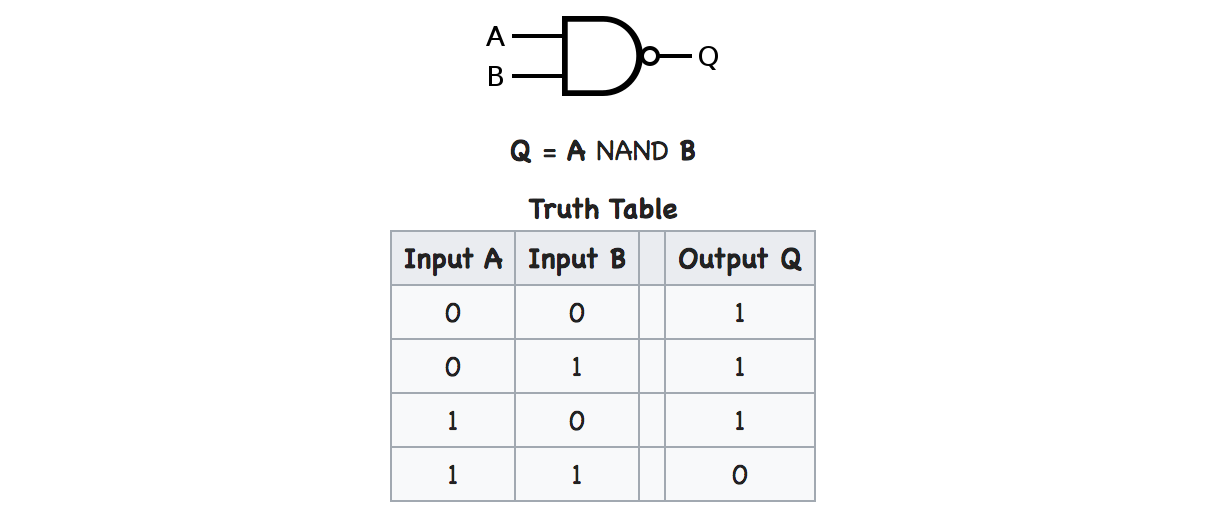
\includegraphics[width=0.5\textwidth]{nand.png}
    \caption{NAND gate and its truth table}
    \label{fig:nand}
\end{figure}

\end{frame}

%%% Introduction to Quantum Computing %%%

\section{Introduction to Quantum Computing}

\subsection{Postulates of Quantum Mechanics}

\begin{frame}{Postulates of Quantum Mechanics}
In the past decades, physicists discover that Nature is "quantum".

    \begin{block}{Mathematical Formulation of the Postulates}
        \begin{itemize}
            \item States of Systems\footnote[frame]{To be more rigorous, closed systems} are Unit Vectors in Hilbert Spaces\footnote[frame]{complete inner product space, e.g. $\mathbb{C}^n$}
            \item Evolutions are linear transforms on the Hilbert space which map states to states.
            \item Measurements are Collections of Operators
            \item States of a Compositional System are Tensor Products of States of Component Systems
        \end{itemize}
    \end{block}

    \begin{exampleblock}{Remark}
        The postulates produces some interesting properties (superposition and entanglement)
    \end{exampleblock}


\end{frame}

\subsection{Notations}
\begin{frame}{Notations}

\begin{itemize}
    \item  In quantum physics, we often use $|\phi\>$ to denote column vector
    \item and use $\<\phi|$ to denote $|\phi\>^\dagger$\footnote{$\dag$ means conjugate transpose}
    \item $\<\phi|\psi\>$ is inner product of $|\phi\>$ and $|\psi\>$
    
\end{itemize}

\end{frame}

\subsection{Quantum Circuit Model}
\begin{frame}{Quantum Circuit Model}

\begin{itemize}
    \item Qubit
    \item Quantum Gate
    \item Oracle
\end{itemize}

\end{frame}

\subsubsection{Qubit}
\begin{frame}{Qubit}

\begin{itemize}
    \item States of Systems are Unit Vectors in Hilbert Spaces
    \item qubit: $|0\>, |1\>$ 
    \item superpostion: $\alpha|0\>+\beta|1\>, |\alpha|^2+|\beta|^2=1$
\end{itemize}

\begin{figure}
    \centering
    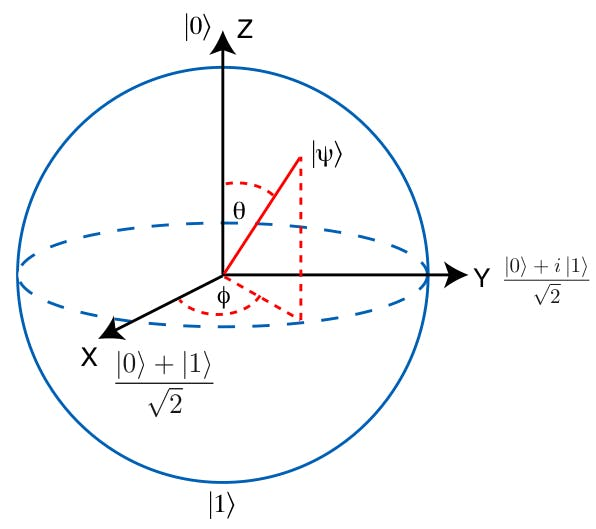
\includegraphics[width=0.4\columnwidth]{bloch.jpg}
    \caption{Bloch Sphere: $|\psi\> = e^{i\delta}(\cos\frac\theta2|0\>+e^{i\phi}\sin\frac\theta2|1\>)$}
    \label{fig:bloch}
\end{figure}

\end{frame}

\note[itemize]{
    \item{why 0, 1}
}

%%%

\subsubsection{Multiple Qubits}
\begin{frame}{Multiple Qubits}

\begin{itemize}
    \item States of a Compositional System are Tensor Products of States of Component Systems
    \item $|00\rangle := |0\rangle \otimes |0\rangle$
    \item $|00\rangle, |01\rangle, |10\rangle, |11\rangle$
    \item n qubit system has $2^n$ bases
\end{itemize}

\end{frame}

%%%

\subsubsection{Quantum Gate}

\begin{frame}{Quantum Gates}
    \begin{itemize}
        \item Evolutions are linear transforms on the Hilbert space which map states to states.
        \item Norm-Preserving + Linear $\implies$ Unitary 
        \item Functions on one qubit: Members of $SU(2) \cong SO(3)$
        \item Like in classical computation, it can be shown that there exists finite universal gate sets\footnote[frame]{\href{https://qudev.phys.ethz.ch/static/content/courses/QSIT07/presentations/Schmassmann.pdf}{ETHZ slide}}
    \end{itemize}
\end{frame}

\note[itemize]{
    \item{"universal" be epsilon-delta argument}
    \item{proof sketch: xzx decomposition + Two Level Gates}
}

\begin{frame}{Quantum Gates --- Examples}

\begin{center}
    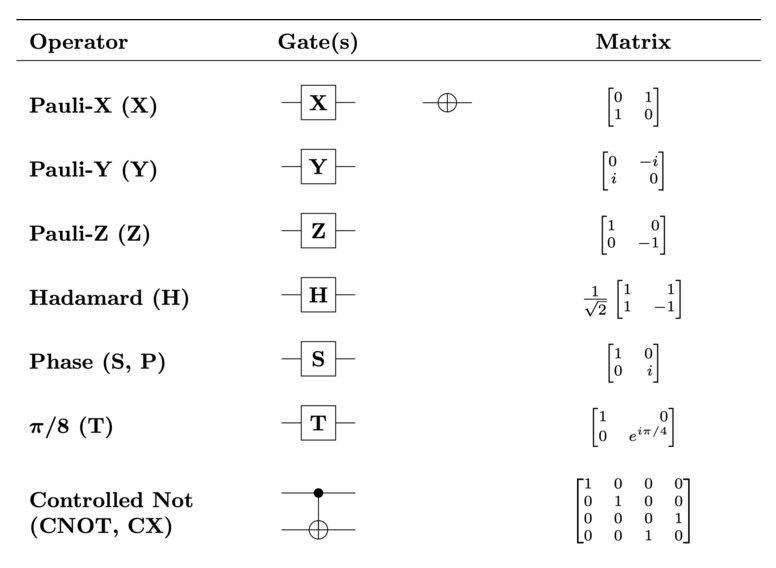
\includegraphics[width=0.8\textwidth]{quantum_gates.png}
\end{center}

\end{frame}
\note[itemize]
{
    \item{Pauli and Clifford}
    \item{X^2=I, H^2=I, HXH=Z, etc.}
    \item{Stabilizer Formalism and T is quantum .}
}

%%%

\subsubsection{Oracle}

\begin{frame}{Oracle}

\begin{itemize}
    \item $O_f$: quantum version of a given function $f$
    \item Requirements
        \begin{itemize}
            \item Unitary
            \item Can be efficiently made up by some finite gate set ($X$ is like $NOT$)
        \end{itemize}
    \item Example
        \begin{itemize}
            \item \sout{$O_f(|x\>) = |f(x)\>$}
            \item $O_f(|x, y\>) = |x, y\oplus f(x)\>$
        \end{itemize}
\end{itemize}

\end{frame}

%%% Quantum Parallelism %%%

\section{Quantum Parallelism}

\subsection{Deutsch-Jozsa Algorithm}
\begin{frame}{A Taste of Power: Quantum Parallelism}

\begin{block}{Problem}
$f:\{0,1\}^n \to \{0,1\}$ is either balanced or constant.
Given $f, O_f$ as black boxes, judge if $f$ is constant.
\end{block}
\begin{itemize}
\item It requires $O(2^n)$ queries of $f$ for a classical circuit to judge
\item quantum: $O(1)$ query
\end{itemize}

\end{frame}

%%

\begin{frame}[allowframebreaks]{Deutsch-Jozsa Algorithm}

\begin{block}{Lemma}
$H^{\otimes n}|z\>=\frac{1}{2^{\frac{n}{2}}}\sum_y (-1)^{y\cdot z}|y\>$
\end{block}

\begin{align*}
 \Qcircuit @C=1em @R=.7em {
  \lstick{\ket{0}} & /^n \qw & \gate{H^{\otimes n}} & \multigate{1}{O_f} & \gate{H^{\otimes n}}	& \meter & \cw \\
  \lstick{\ket{1}} & \qw     & \gate{H}             & \ghost{U_f}        & \qw
 }
\end{align*}

\framebreak

\footnotesize

$$\vert \psi_0 \rangle = \vert0\rangle^{\otimes n} \vert 1\rangle$$
$$\vert \psi_1 \rangle = \frac{1}{\sqrt{2^{n+1}}}\sum_{x=0}^{2^n-1} \vert x\rangle \left(|0\rangle - |1 \rangle \right)$$
$$
    \begin{aligned}
    \lvert \psi_2 \rangle  
        & = \frac{1}{\sqrt{2^{n+1}}}\sum_{x=0}^{2^n-1} \vert x\rangle (\vert f(x)\rangle - \vert 1 \oplus f(x)\rangle) \\  
        & = \frac{1}{\sqrt{2^{n+1}}}\sum_{x=0}^{2^n-1}(-1)^{f(x)}|x\rangle ( |0\rangle - |1\rangle ) 
    \end{aligned}
$$
$$
\begin{aligned}
    \lvert \psi_3 \rangle 
        & = \frac{1}{2^n}\sum_{x=0}^{2^n-1}(-1)^{f(x)}
            \left[ \sum_{y=0}^{2^n-1}(-1)^{x \cdot y} 
            \vert y \rangle \right] \\
        & = \frac{1}{2^n}\sum_{y=0}^{2^n-1}
            \left[ \sum_{x=0}^{2^n-1}(-1)^{f(x)}(-1)^{x \cdot y} \right]
            \vert y \rangle
\end{aligned}
$$

\normalsize

\framebreak

Now consider $|y\>=|0\>$
$$
\frac{1}{2^n}\sum_{x=0}^{2^n-1}(-1)^{f(x)}(-1)^{x \cdot 0}
            \vert 0 \rangle
$$
\begin{block}{Question}
Why does this work?
\uncover<1->{interference!}
\end{block}

\end{frame}

%%%%



%%% Grover's Search %%%

\section{Grover's Search}

\subsection{Problem Definition}
\begin{frame}
\frametitle{Problem Definition}

\begin{block}{Unstructured Search}
Given a set $X$ of $N$ items and a function $f : X \to \{0,1\}$, \newline
suppose there are $M=\epsilon N$ out of $N$ items satisfy $f(x)=1$. \newline
Find an instance $x \in S$ such that $f(x)=1$. \newline
\end{block}

\begin{itemize}
    \item For classical algorithms, $O(N)$-time is required to get an instance with high probability.

    \item For quantum algorithms, assume an oracle $U_\omega$ is given such that 
$$
U_\omega|x\rangle = (-1)^{f(x)}|x\rangle .
$$
    With Grover's Search, $O(\sqrt{N})$-time is suffice.
\end{itemize}

\end{frame}


\subsection{the Good/Bad basis}
\begin{frame}
\frametitle{the Good/Bad basis}
Represent uniform state vector by l.c. of uniform "good" and uniform "bad" vectors. \newline
$|s\rangle = \sqrt{\frac{1}{N}}\sum_{x} |x\rangle$ \newline
$|\omega\rangle = \sqrt{\frac{M}{N}}\sum_{x \in f^{-1}(1)} |x\rangle$ \newline
$|s^{'}\rangle = \sqrt{\frac{N-M}{N}}\sum_{x \not \in f^{-1}(1)} |x\rangle$ \newline
then $|s\rangle = \sin\frac\theta2|\omega\rangle + \cos\frac\theta2|s^{'}\rangle$ where $\sin\frac\theta2 = \sqrt{\frac{M}{N}}$
\end{frame}


\subsection{Geometric Intuition}
\begin{frame}{Geometric Intuition}

\begin{figure}
    \centering
    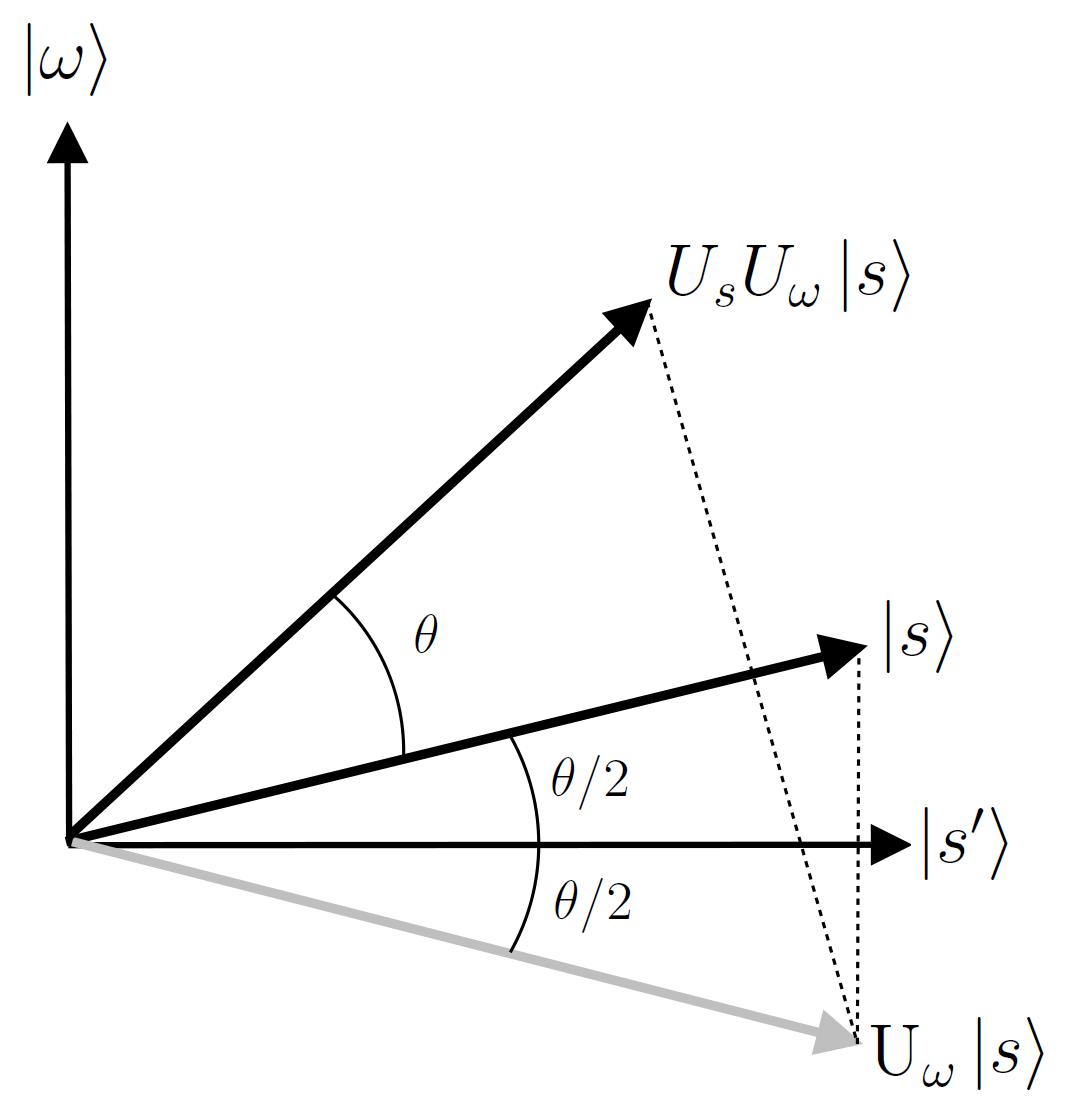
\includegraphics[width=0.5\columnwidth]{grover_geo.png}
    \caption{One step of Grover's Iteration: Rotation by $\theta$ }
    \label{fig:grover_geo}
\end{figure}

\end{frame}

\subsection{Complexity}
\begin{frame}{Complexity}

We want to stop when the state vector passes close to $|\omega \rangle$. \newline
Suppose Grover's iteration is performed $r$ times, the probability of success is exactly $\sin^2\left( \Big( r + \frac{1}{2} \Big)\theta\right)$. \newline
$r\approx \pi \sqrt {N}/4$ is the first $r$ we can get a high probability.

\end{frame}

\subsection{Implementation}
\begin{frame}
\frametitle{Implementation}
$$U_\omega = I - 2|\omega\rangle\langle \omega|$$
$$U_s = 2 \left|s\right\rangle \left\langle s\right| - I$$

\begin{align*}
 \Qcircuit @C=1em @R=.7em {
                   &         &                      &                         &                      & \ustick{\text{Grover diffusion operator $U_s$}} \\
  \lstick{\ket{0}} & /^n \qw & \gate{H^{\otimes n}} & \multigate{1}{U_\omega} & \gate{H^{\otimes n}} & \gate{2 \ket{0^n}\bra{0^n} - I_n}         & \gate{H^{\otimes n}} & \qw & \cdots & & \meter & \cw \\
  \lstick{\ket{1}} & \qw     & \gate{H}             & \ghost{U_\omega}        & \qw                  & \qw                                       & \qw                  & \qw & \cdots & \\
                   &         &                      &                         &                      & \dstick{\text{Repeat $O(\sqrt{N})$ times}}
  \gategroup{2}{5}{2}{7}{.7em}{^\}}
  \gategroup{2}{4}{3}{10}{.7em}{_\}}
 }
\end{align*}

\end{frame}


%%%% Concluding Remarks

\section{Concluding Remarks}
\begin{frame}
\frametitle{Concluding Remarks}
\begin{itemize}
    \item Amazing algorithms like Shor's factoring algorithm
    \item Quantum Fourier Transformation and Quantum Phase Estimation
    \item Quantum Walks, the generalization of Grover's Search
    \item QAOA for solving CSP problems
\end{itemize}
\end{frame}

\end{document}